\documentclass[border=10pt]{standalone}
\usepackage{amsmath}
\usepackage{tikz}

\begin{document}
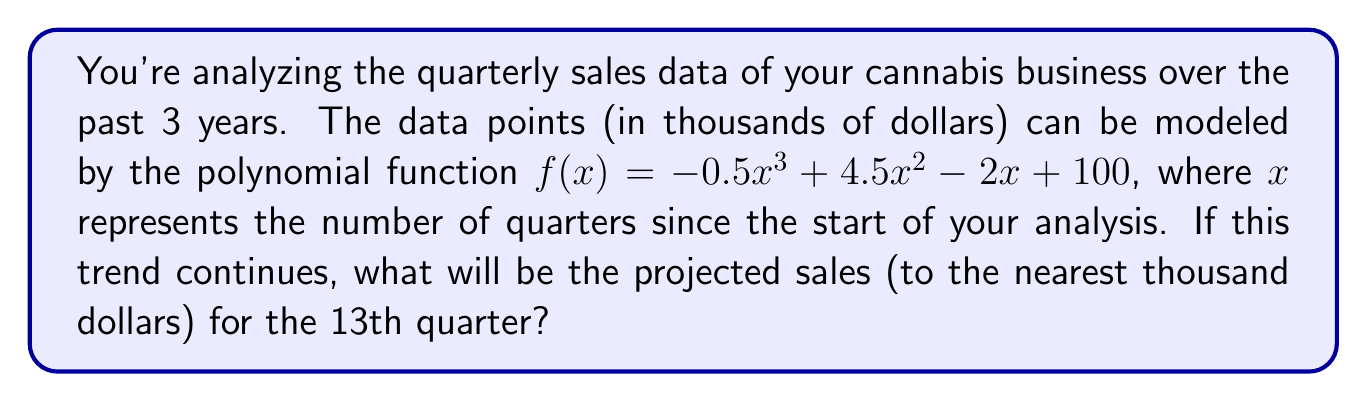
\begin{tikzpicture}
    \node[
        draw=blue!60!black,
        fill=blue!8,
        line width=1.5pt,
        rounded corners=10pt,
        text width=15.4cm,
        align=justify,
        inner xsep=0.6cm,
        inner ysep=0.35cm,
        font=\sffamily\Large
    ] at (0,0) {
        You're analyzing the quarterly sales data of your cannabis business over the past 3 years. The data points (in thousands of dollars) can be modeled by the polynomial function \( f(x) = -0.5x^3 + 4.5x^2 - 2x + 100 \), where \( x \) represents the number of quarters since the start of your analysis. If this trend continues, what will be the projected sales (to the nearest thousand dollars) for the 13th quarter?
    };
\end{tikzpicture}
\end{document}
